\documentclass[handout]{beamer}

\usepackage{Haust2017glærur}

\title{Stærðfræðimynstur í tölvunarfræði}
\subtitle{Vika 8, fyrri fyrirlestur}

\begin{document}

\begin{frame}
\titlepage
\end{frame}


\section{Inngangur}

\begin{frame}{Í síðasta tíma}
    \begin{itemize}
        \item Umraðanir
        \item Samantektir
        \item Tvíliður
    \end{itemize}
\end{frame}

\section{Miðmisseriskönnun og viðbrögð}

\begin{frame}{Miðmisseriskönnun}
    \begin{center}
        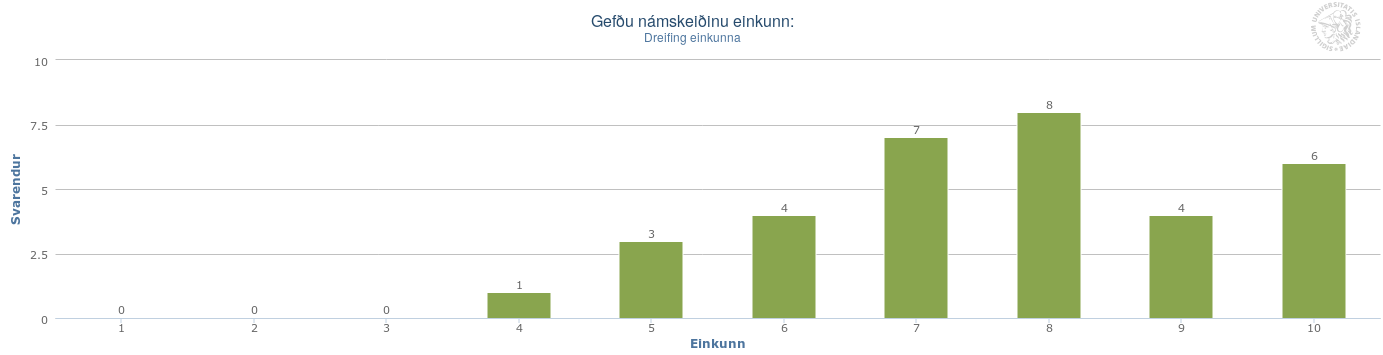
\includegraphics[width=\textwidth]{Dreifing2017}
    \end{center}
    121 af 229 tóku þátt ($\approx 53\%$). Meðaleinkunn 6.93 (Meðaleinkunn IVT 7.8).
\end{frame}

\begin{frame}{Almenn ánægja}
    \begin{itemize}
        \item Fleiri jákvæðar en neikvæðar athugasemdir bárust um
        \begin{itemize}[<+->]
            \item Upptökur
            \item Dæmatímakennarana
            \item Skilaverkefnin (mikil bót frá í fyrra)
            \item Piazza og Connect
            \item Persónu aðalkennarans
        \end{itemize}
    \end{itemize}
\end{frame}

\begin{frame}{Skiptar skoðanir}
    \begin{itemize}[<+->]
        \item Gradescope
        \begin{itemize}
            \item Kerfið er frábært
            \item Kerfið er meingallað
            \begin{itemize}
                \item Regrade requests skila sér ekki
            \end{itemize}
        \end{itemize}
        \item Sýnidæmi
        \begin{itemize}
            \item Ættu ekki að vera öll úr bókinni
            \item Tengjast dæmunum úr bókinni ekki nóg
        \end{itemize}
        \item Hraði yfirferðar
        \begin{itemize}
            \item Of hröð
            \item Of hæg
        \end{itemize}
    \end{itemize}
\end{frame}

\begin{frame}{Má betur fara}
    \begin{itemize}
        \item Yfirferð á skilaverkefnum
        \item Þurrt efni
        \item Samhengisleysi, vaðið úr einu í annað
        \item Hentar ekki fólki með stærðfræðibakgrunn
    \end{itemize}
\end{frame}

\begin{frame}{Hugmyndir að aðgerðum}
    \begin{itemize}
        \item Dæmayfirferðin verður skoðuð á fundi með dæmatímakennurum
        \item Staða stærðfræðinema innan námskeiðsins verður skoðuð með námsbrautarformönnum
    \end{itemize}
\end{frame}

\section{Vensl}

\begin{frame}{Upprifjun - Mengjamargfeldi}
\begin{tcolorbox}[title=Mengjamargfeldi]
Látum $A$ og $B$ vera mengi. Mengjamargfeldi $A$ og $B$ er mengi allra raðaðra para $(a, b)$ þar sem $a \in A$ og $b \in B$, þ.e.a.s. mengið $\{(a, b) | a \in A \land b \in B\}$. Mengjamargfeldi $A$ og $B$ er táknað með $A \times B$.
\end{tcolorbox}
Dæmi:
\[
 \{1, 2\} \times \{a, b\} = \pause \{(1, a), (1, b), (2, a), (2, b)\}
\]
Athugum að almennt gildir ekki að $A \times B$ sé jafnt $B \times A$.
\end{frame}

\begin{frame}{Tvíundarvensl}
Getum skilgreint vensl (e. \emph{relation}) frá einu mengi til annars.

\begin{tcolorbox}[title=Tvíundarvensl]
Látum $A$ og $B$ vera mengi. Tvíundarvensl (e. \emph{binary relation}) frá $A$ til $B$ er hlutmengi í $A \times B$.
\end{tcolorbox}
Sé $a \in A$, $b \in B$ og $R$ vensl frá $A$ til $B$ skrifum við $a$ $R$ $b$ sé $(a,b) \in R$.

\vspace{0.5cm}

Hugmyndin - venslin mynda einhvers konar ``tengingu'' á milli mengjanna
\end{frame}

\begin{frame}{Dæmi}
Látum $A$ vera mengi nemenda við HÍ og $B$ vera mengi námskeiða við HÍ. Þá getum við látið $R$ vera venslin sem innihalda þau pör $(a,b)$ þar sem nemandi $a \in A$ er skráður í námskeið $b \in B$.
\end{frame}

\begin{frame}{Framsetning á venslum}
\begin{columns}
\column{0.5\textwidth}
Látum $A = \{0, 1, 2\}$ og $B = \{a, b\}$. Þá er $R = \{(0,a), (0,b), (1,a), (2,b)\}$ vensl frá $A$ til $B$. 

Þá er t.d. $0$ $R$ $a$.

Við getum sett þessi vensl fram með t.d. örvamynd eða töflu.
\column{0.5\textwidth}
\begin{center}
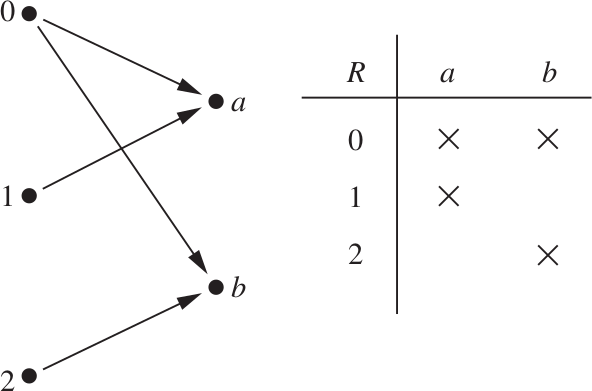
\includegraphics[width=\linewidth]{relation-visualization}
\end{center}
\end{columns}
\end{frame}

\begin{frame}{Vensl og föll}
\begin{itemize}
 \item Munum að fall $f$ með $A$ sem formengi og $B$ sem bakmengi skilgreinir nákvæmlega eitt $b \in B$ fyrir hvert $a \in A$
 \begin{itemize}
  \item Graf fallsins (e. \emph{the graph of the function}) $f$ er þá mengi raðaðra para $(a, b)$ svo að $f(a) = b$.
  \item Graf fallsins er þá hlutmengi $A\times B$, svo það er vensl frá $A$ til $B$
 \end{itemize}
 \item Vensl geta lýst sambandi þar sem hvert stak í $A$ tengist meira en einu staki í $B$
 \begin{itemize}
  \item Vensl geta lýst almennara sambandi en fall (eða öllu heldur graf falls)
\end{itemize}
\end{itemize}
\end{frame}

\begin{frame}{Vensl á mengi}
Vensl frá mengi $A$ yfir í sjálft sig koma oft fyrir.

\begin{tcolorbox}[title=Vensl á mengi]
Vensl á mengi (e. \emph{relation on a set}) $A$ eru vensl frá menginu $A$ til $A$. 
\end{tcolorbox}

Sem sagt, vensl á mengi $A$ er hlutmengi í $A \times A$.
\end{frame}

\begin{frame}{Fjöldi vensla á mengi}
    \begin{itemize}
        \item Hversu mörg vensl eru til á mengi $A$ með $n$ stökum?\pause
        \item $A \times A$ hefur þá $n^2$ stök (sjá: margfeldisregla) \pause
        \item Mengi með $m$ stökum hefur $2^m$ hlutmengi \pause
        \item Til eru $2^{n^2}$ vensl á $n$ staka mengi
    \end{itemize}
\end{frame}

\begin{frame}{Dæmi}
Getum séð fyrir okkur vensl á mengi heiltalna ($a, b \in Z$)
\begin{align*}
R_1 &= \{(a, b)|a \leq b\}\\
R_2 &= \{(a, b)|a > b\}\\
R_3 &= \{(a, b)|a = b \text{ eða } a = -b\}\\
R_4 &= \{(a, b)|a = b\}\\
R_5 &= \{(a, b)|a = b+1\}\\
R_6 &= \{(a, b)|a+b \leq 3\}\\
\end{align*}
Hér er um að ræða vensl á óendanlegt mengi. Venslin sjálf eru óendanleg mengi.
\end{frame}

\subsection{Eiginleikar vensla}

\begin{frame}{Sjálfhverf vensl}
\begin{tcolorbox}[title=Sjálfhverf vensl]
Vensl $R$ á mengi $A$ eru sjálfhverf (e. \emph{reflexive}) þá og því aðeins að $(a, a) \in R$ fyrir hvert $a \in A$.
\end{tcolorbox}
\vspace{0.5cm}
\begin{columns}
\column{0.5\textwidth}
Sjálfhverf vensl:
\begin{align*}
R_1 &= \{(a, b)|a \leq b\}\\
R_3 &= \{(a, b)|a = b \text{ eða } a = -b\}\\
R_4 &= \{(a, b)|a = b\}\\
\end{align*}
\column{0.5\textwidth}
Ekki sjálfhverf vensl:
\begin{align*}
R_2 &= \{(a, b)|a > b\}\\
R_5 &= \{(a, b)|a = b+1\}\\
R_6 &= \{(a, b)|a+b \leq 3\}\\
\end{align*}
\end{columns}
\end{frame}

\begin{frame}{Samhverf vensl}
\begin{tcolorbox}[title=Samhverf vensl]
Vensl $R$ á mengi $A$ eru samhverf (e. \emph{symmetric}) ef $(b, a) \in R$ hvenær sem $(a,b) \in R$ fyrir öll $a,b \in A$. Þ.e.a.s. $R$ eru samhverf vensl á $A$ ef $\forall a \forall b ((a,b) \in R \to (b, a) \in R)$.
\end{tcolorbox}
\vspace{0.5cm}
\begin{columns}
\column{0.5\textwidth}
Samhverf vensl:
\begin{align*}
R_3 &= \{(a, b)|a = b \text{ eða } a = -b\}\\
R_4 &= \{(a, b)|a = b\}\\
R_6 &= \{(a, b)|a+b \leq 3\}\\
\end{align*}
\column{0.5\textwidth}
Ekki samhverf vensl:
\begin{align*}
R_1 &= \{(a, b)|a \leq b\}\\
R_2 &= \{(a, b)|a > b\}\\
R_5 &= \{(a, b)|a = b+1\}\\
\end{align*}
\end{columns}
\end{frame}

\begin{frame}{Samhverf vensl utan stærðfræðinnar}
    \begin{itemize}
        \item ``Er jafngilt''
        \begin{itemize}
            \item Jafngildisvensl: Vensl sem eru samhverf, sjálfhverf og gegnvirk
        \end{itemize}
        \item ``Er í hjónabandi með'' (skv. íslenskum lögum)
        \item ``Er systkini''
    \end{itemize}
\end{frame}

\begin{frame}[fragile]{Andsamhverf vensl}
\begin{tcolorbox}[title=Andsamhverf vensl]
Vensl $R$ á mengi $A$ eru andsamhverf (e. \emph{antisymmetric}) ef fyrir öll $a, b \in A$ gildir að ef $(a, b) \in R$ og $(b, a) \in R$, þá er $a=b$. Þ.e.a.s. vensl $R$ á mengi $A$ eru andsamhverf ef\\ $\forall a \forall b (((a, b) \in R \land (b, a) \in R) \to (a = b))$.
\end{tcolorbox}
Ath: hugtökin ``samhverf'' og ``andsamhverf'' eru ekki andstæður.
\begin{columns}
\column{0.5\textwidth}
Andsamhverf vensl:
\begin{align*}
R_1 &= \{(a, b)|a \leq b\}\\
R_2 &= \{(a, b)|a > b\}\\
R_4 &= \{(a, b)|a = b\}\\
R_5 &= \{(a, b)|a = b+1\}\\
\end{align*}
\column{0.5\textwidth}
Ekki andsamhverf vensl:
\begin{align*}
R_3 &= \{(a, b)|a = b \text{ eða } a = -b\}\\
R_6 &= \{(a, b)|a+b \leq 3\}\\
\end{align*}
\end{columns}
\end{frame}

\begin{frame}[fragile]{Gegnvirk vensl}
\begin{tcolorbox}[title=Gegnvirk vensl]
Vensl $R$ á mengi $A$ eru gegnvirk (e. \emph{transitive}) ef, hvenær sem $(a, b) \in R$ og $(b, c) \in R$, þá sé $(a, c) \in R$, fyrir öll $a, b, c \in A$. Þ.e.a.s. vensl $R$ á mengi $A$ eru gegnvirk þegar $\forall a\forall b\forall c(((a, b) \in R \land (b, c) \in R) \to (a, c) \in R)$
\end{tcolorbox}
\begin{columns}
\column{0.5\textwidth}
Gegnvirk vensl:
\begin{align*}
R_1 &= \{(a, b)|a \leq b\}\\
R_2 &= \{(a, b)|a > b\}\\
R_3 &= \{(a, b)|a = b \text{ eða } a = -b\}\\
R_4 &= \{(a, b)|a = b\}\\
\end{align*}
\column{0.5\textwidth}
Ekki gegnvirk vensl:
\begin{align*}
R_5 &= \{(a, b)|a = b+1\}\\
R_6 &= \{(a, b)|a+b \leq 3\}\\
\end{align*}
\end{columns}
\end{frame}

\begin{frame}{Gegnvirkni in the wild}
    Hluti af skilgreiningu ``Comparable Interface'' í Java
    \begin{center}
        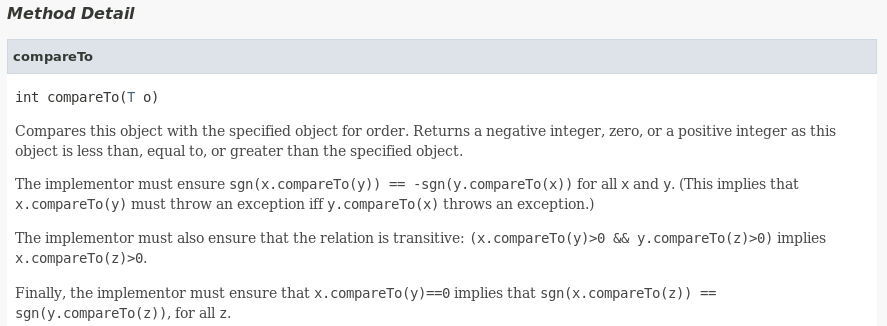
\includegraphics[width=\textwidth]{compareTo}
    \end{center}
    Kemur við sögu í Tölvunarfræði 2.
\end{frame}

\begin{frame}{Samsetning vensla}
\begin{tcolorbox}[title=Samsetning vensla]
Látum $R_1$ vera vensl frá mengi $A$ til mengis $B$ og $R_2$ vera vensl frá $B$ til mengis $C$. Þá skilgreinum við samsettu venslin $R_1 \circ R_2$ með eftirfarandi:

$(x,z) \in R_1 \circ R_2$ þá og því aðeins að til sé $y \in B$ þannig að $(x,y) \in R_1$ og $(y,z) \in R_2$.
\end{tcolorbox}
\end{frame}

\begin{frame}{Samsetning - myndrænt}
\begin{center}
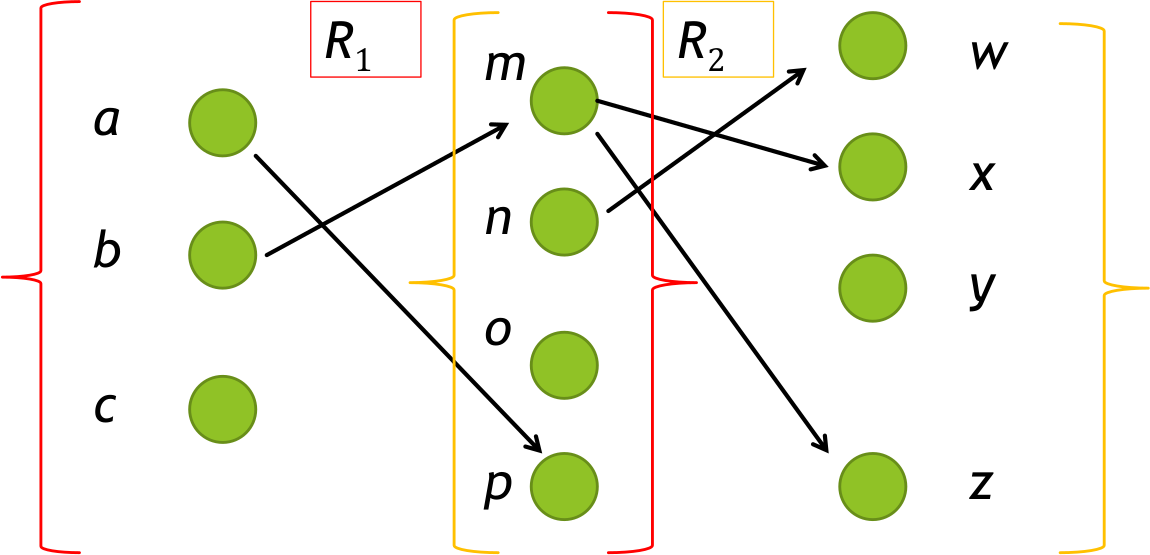
\includegraphics[width=\textwidth]{combined-relation}
\end{center}
\end{frame}

\begin{frame}{Dæmi}
Hver eru samsettu venslin $S \circ R$ þegar $R$ er frá $\{1, 2, 3\}$ til $\{1, 2, 3, 4\}$ með $R = \{(1, 1), (1, 4), (2, 3), (3, 1), (3, 4)\}$ og $S$ er frá $\{1, 2, 3, 4\}$ til $\{0, 1, 2\}$ með $S = \{(1, 0), (2, 0), (3, 1), (3, 2), (4, 1)\}$? \pause 

\vspace{0.5cm}
Finnum öll röðuð pör þar sem seinna stakið í pari úr $R$ passar við fyrra stakið úr $S$. Fáum:
\[
 S \circ R = \{(1, 0), (1, 1), (2, 1), (2, 2), (3, 0), (3, 1)\}
\]
\end{frame}

\begin{frame}{Næst}

Kafli 9.2 (Hagnýting vensla), kafli 9.3 (Framsetning vensla).

E.t.v. gagnlegur kafli til dýpkunar á kafla 9.3: Kafli 10.1 (Net)

\end{frame}


\end{document}
